%!TEX root = ./template-skripsi.tex

\subsection{\textit{Sprint 5}}

	\textit{Sprint-5} dilakukan sepekan pada tanggal 20 September 2022 sampai dengan 27 september 2022. \textit{Story} kelimat pada \textit{product backlog} yaitu membuat fitur rekapitulasi kematian ikan dipecah menjadi beberapa \textit{task} sebagai berikut.


 \begin{longtable}[c]{@{} |p{1cm}|p{4cm}|p{5cm}|p{3cm}| @{}}
 \caption{\textit{Sprint 5} \label{sprint5_table}}\\


 \hline
  \multirow{1}{=}{\centering{\textbf{No}}} & \multirow{1}{=}{\centering{\textbf{\textit{Story}}}} & \multirow{1}{=}{\centering{\textbf{\textit{Task}}}} & \multirow{1}{=}{\centering{\textbf{\textit{Status}}}}\\
 \endfirsthead

 \hline
  \multirow{1}{=}{\centering{\textbf{No}}} & \multirow{1}{=}{\centering{\textbf{\textit{Story}}}} & \multirow{1}{=}{\centering{\textbf{\textit{Task}}}} & \multirow{1}{=}{\centering{\textbf{\textit{Status}}}}\\
 \endhead

 \hline
 \endfoot

 \hline
 \endlastfoot

 \hline
 1 & Membuat fitur rekapitulasi kematian ikan &  Membuat \textit{Mock-up UI} halaman rekapitulasi kematian ikan, entry kematian ikan  &  selesai \\
 \hline
 2 & & Menerapkan \textit{Mock-up UI} halaman rekapitulasi kematian ikan, entry kematian ikan ke Flutter & selesai\\
 \hline
 3 & & Mengintegrasikan halaman rekapitulasi kematian ikan, entry kematian ikan ke \textit{webservice} & selesai\\
 \hline
 \end{longtable}

Pada sprint kelima ini story yang di pilih untuk di uraikan pada sprint kali ini adalah membuat halaman rekapitulasi kematian ikan, entry kematian ikan. Tujuan dari \textit{sprint-5} ini adalah membuat fitur rekapitulasi kematian ikan dan mengintegrasikan halaman tersebut dengan webservice yang sudah dibuat oleh penelitian Andri Rahmanto.

\begin{enumerate}[listparindent=2em]
	
	\item{\textit{Membuat Mock-up UI Fitur Rekapitulasi Kematian Ikan}}
	
	Pembuatan konten dan fitur yang terdapat pada \textit{mock-up UI} fitur rekapitulasi kematian ikan dilakukan berdasarkan persetujuan product owner dan scrum master pada meeting sebelumnya. Mock-up UI dibuat menggunakan platform figma.
	
	\begin{figure}[H]
	\centering
	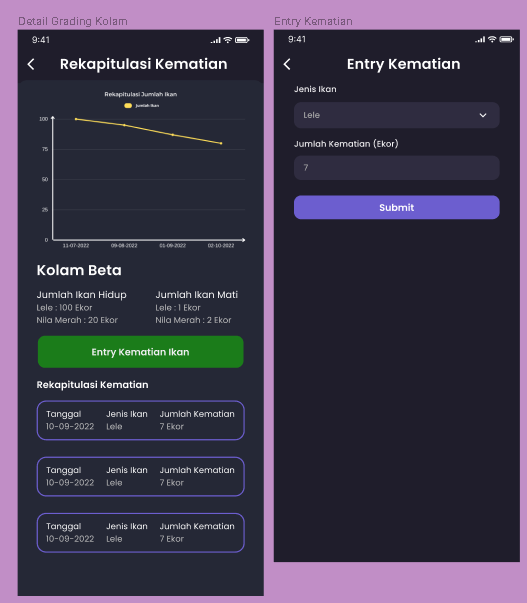
\includegraphics[keepaspectratio, width=6cm]{gambar/mockupkematian}
	\caption{\textit{Mock-up UI Fitur Rekapitulasi Kematian Ikan}}
	\label{gambar:mockupkematian}
	\end{figure}

	\item{\textit{Class Diagram}}
	
	Class Diagram menggambarkan kelas-kelas yang akan dipakai oleh sistem. Umumnya terdapat 3 kelas pada setiap module yaitu class model, controller, dan view. Pada sprint-5 penelitian kali ini penulis membuat 4 class yaitu model yang berwarna biru, view berwarna oranye, controller yang berwarna hijau, dan service yang berwarna kuning.
	 
	 \begin{figure}[H]
	 \centering
	 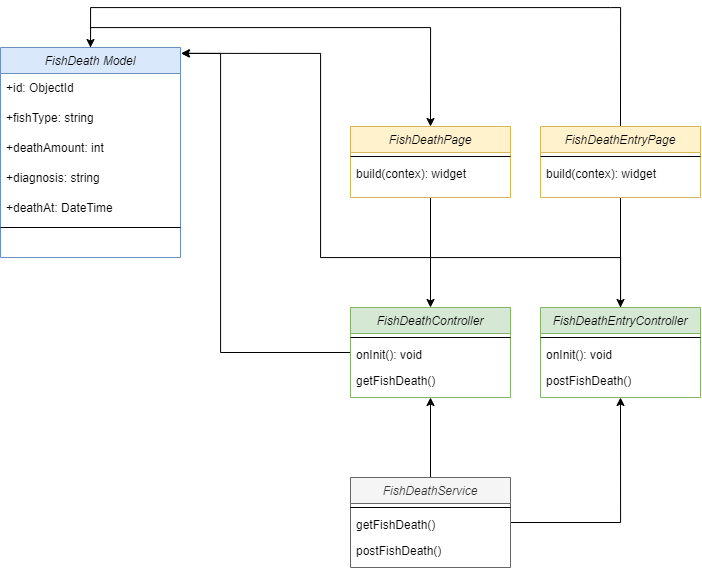
\includegraphics[keepaspectratio, width=6cm]{gambar/deathcd}
	 \caption{\textit{Class Diagram Fitur Sprint-5}}
	 \label{gambar:deathcd}
	 \end{figure}

	\item{\textit{Menerapkan Mockup-UI fitur rekapitulasi kematian ikan kedalam code flutter}}
	
	Setelah itu, akan dilakukan pengimplementasian \textit{mock-up UI} ke dalam aplikasi menggukan flutter. Pada lampiran 6 source code dari implementasi fitur grading yang dikelompokan berdasarkan halaman yang menghasilkan output halaman seperti dibawah ini.

	\begin{figure}[H]
		\centering
		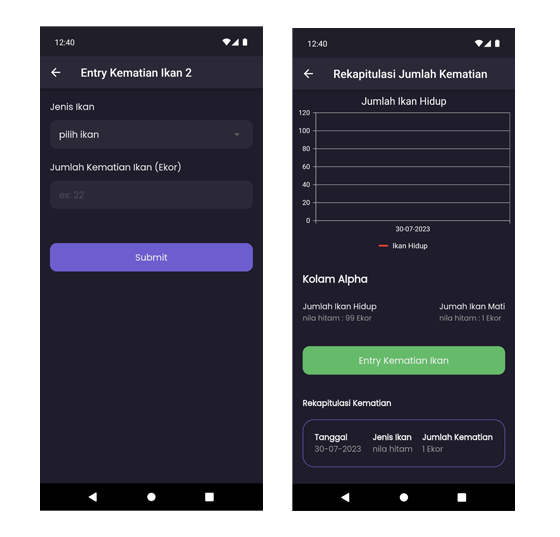
\includegraphics[keepaspectratio, width=8cm]{gambar/sssprint5}
		\caption{\textit{Output dari code pada sprint 5}}
		\label{gambar:sssprint5}
		\end{figure}

	\item{\textit{Mengitegrasikan fitur rekapitulasi kematian dengan webservice}}

	Sebelumnya, setiap data pada fitur masih berupa data dummy sehingga perlu diintegrasikan dengan webservice agar aplikasi dapat berjalan dengan data yang asli. Hal yang dilakukan dalam mengintegrasikan fitur rekapitulasi kematian ikan dengan webservice terdapat pada lampiran 6.

  \item{Analisis \textit{User Experience}} 
 
  Pada halaman entry rekapitulasi kematian, pembudidaya harus jenis ikan dan data jumlah kematian. Di halaman rekapitulasi kematian, terdapat grafik mengenai statistik jumlah ikan  pada musim budidaya yang berjalan sehingga pembudidaya dapat dengan mudah mengetahui penurunan jumlah ikan akibat kematian. Selain itu terdapat juga list mengenai data kematian yang telah dimasukan yang berisi informasi yang berhubungan dengan kematian ikan.

\item{Sprint 5 Review dan Sprint 6 Planning}

Sprint 5 diakhiri dengan melakukan weekly meeting pada hari selasa dengan agenda melakukan review dan testing terkait hasil sprint 5 dan melakukan planning untuk sprint 6 dengan rincian:
\begin{enumerate}
	\item{\textit{Review dan Testing hasil dari sprint 5}}

	Telah dilakukan review dan testing oleh penulis selaku developer dengan Scrum Master. Setelah dilakukan testing, Scrum Master menyimpulkan bahwa fitur rekapitulasi kematian ikan telah berjalan dengan baik.
	
  \begin{longtable}{| p{8cm} | c | c | l |}
    \caption{Unit testing Halaman Rekapitulasi Kematian.\label{table:unit_testing_rekapitulasi_kematian}}\\
    \hline
    \multirow{2}{*}{Skenario Pengujian} & \multicolumn{2}{l|}{Kesesuaian} & \multirow{2}{*}{Kesimpulan} \\ 
    \cline{2-3}
      & \multicolumn{1}{l|}{sesuai} & tidak sesuai & \\ 
    \hline
    \hline
    \endfirsthead
    \hline
    \multirow{2}{*}{Skenario Pengujian} & \multicolumn{2}{l|}{Kesesuaian} & \multirow{2}{*}{Kesimpulan} \\ 
    \cline{2-3}
      & \multicolumn{1}{l|}{sesuai} & tidak sesuai &  \\ 
    \hline
    \hline
    \endhead
    \hline
    \endfoot
    
    
    \hline\hline
    \endlastfoot
    Ketika menekan list data rekapitulasi pakan, maka akan ditamplikan detail rekapitulasi pakan & \Checkmark &  & Diterima \\ 
    \hline
    Saat tombol entry kematian ditekan maka akan menampilkan halaman entry kematian & \Checkmark &  & Diterima \\ 
    \hline
    ketika mengisi form rekapitulasi kematian dengan data yang sesuai dan menekan submit, data rekapitulasi kematian akan ditambahkan & \Checkmark &  & Diterima \\ 
    \hline
    \end{longtable}

	\item{\textit{Sprint Planning untuk Sprint 6}}
	
	Planning untuk sprint 6 yakni membuat fitur treatment kolam pada aplikasi \textit{Assistive Aquaculture Breeding Management}.
\end{enumerate}
\end{enumerate}